\documentclass{classrep}
\usepackage[utf8]{inputenc}
\frenchspacing

\usepackage{graphicx}
\usepackage[usenames,dvipsnames]{color}
\usepackage[hidelinks]{hyperref}
\usepackage{lmodern}
\usepackage{placeins}
\usepackage{url}
\usepackage{amsmath, amssymb, mathtools}
\usepackage{listings}
\usepackage{fancyhdr, lastpage}

\pagestyle{fancyplain}
\fancyhf{}
\renewcommand{\headrulewidth}{0pt}
\cfoot{\thepage\ / \pageref*{LastPage}}

%--------------------------------------------------------------------------------------%
\studycycle{Informatyka stosowana, studia dzienne, II st.}
\coursesemester{II}

\coursename{Analiza danych złożonych}
\courseyear{2021/2022}

\courseteacher{dr hab inż. Agnieszka Duraj}
\coursegroup{środa, 11:00}

\author{%
    \studentinfo[239671@edu.p.lodz.pl]{Jan Karwowski}{239671}\\
    \studentinfo[239676@edu.p.lodz.pl]{Kamil Kowalewski}{239676}\\
}

\title{Zadanie 5.: Metody oparte na logice rozmytej}

\begin{document}
    \maketitle
    \thispagestyle{fancyplain}

    \tableofcontents
    \newpage

    \section{Cel} {
        Celem zadania jest sprawdzenie działania logiki rozmytej w wykrywaniu wyjątków
        dla trzech zbiorów danych przy wykorzystaniu wybranych algorytmów.
    }

    \section{Zbiory danych} {
        Do przeprowadznia badań w tym zadaniu zostały wykorzystane trzy zbiory danych,
        dwa z nich są zbiorami naturalnymi natomiast jeden z nich jest sztucznie
        wygenerowany.

        Zbiór wygenerowany sztucznie został utworzony poprzez wykorzystanie funkcji
        \textit{generate\_data}, która jest wbudowana w bibliotekę
        \textit{PyOD}\cite{pyod}. Zbiór ten ma 2 wymiary natomiast procent wyjątków
        został ustawiony na wartość równą \textit{10\%}.

        Drugi i trzeci zbiór danych pochodzą z serwisu \emph{Outlier Detection DataSets}
        \cite{odds}, który zawiera kilkadziesiąt przykładowych zbiorów
        danych, dostosowanych do zadania wyszukiwania wyjątków. Zbiory te są już
        znormalizowane i oczyszczone, każdy przykład w każdym zbiorze jest oznaczony
        jedną z dwóch klas: wyjątek lub nie wyjątek. Wybranymi zbiorami są ,,http''
        oraz ,,mammography''.

        Zbiór ,,http'' zawiera 3 kolumny i oryginalnie ponad 500 tys. wierszy, z czego
        ok. 0.4\% stanowią wyjątki. Zbiór ten na potrzebny niniejszego zadania został
        ograniczony do ok 1\% próbek, przy czym proporcja wyjątków została zachowana.
        Zbiór ten zawiera informacje o zapytaniach HTTP.

        Zbiór ,,mammography'' zawiera 6 kolumn i ponad 11 tys. wierszy, z czego ok. 2\%
        stanowią wyjątki. Zbiór ten dotyczy wyników badania mammograficznego i
        wyjątkami są przypadki zdiagnozowane jako chore, których jest stosunkowo mało
        do przypadków zdrowych, przez co zbiór ten został dostosowany do zadania
        rozpoznawania wyjątków, chociaż oryginalnie dotyczy zadania klasyfikacji.
    }

    \section{Implementacja} {
        Program został napisany w języku Python z wykorzystaniem biblioteki
        \textit{fuzzy-c-means}\cite{fuzzy_c_means} aby skorzystać z gotowych
        implementacji algorytmów. Wybranym algorytmem jest:
        \begin{itemize}
            \item Fuzzy CMeans
        \end{itemize}

        Do porównania wyników został wykorzystany algorytm KMeans dostępny w bibliotece
        \textit{scikit-learn}\cite{sklearn}.

        Do kodu źródłowego jest dołączony skrypt \textit{run.sh} zawierający wszystkie
        kombinacja parametrów użyte do badań natomiast wyniki w postaci wykresów są
        zapisywane do plików.
    }

    \section{Opis algorytmów} {

        \subsection{KMeans} {
            Algorytm K-średnich należy do metody grupowania opartego na odległości.
            Jego działania rozpoczyna się od podziału zbioru przypadku na \textit{K}
            skupień i rozpoczyna działanie od losowo wybranych \textit{K} środków
            skupień, które są możliwie jak najbardziej od siebie oddalone. W czasie
            kolejnych iteracji przypisuje obiekty do najbliższych skupień. Sama
            odległość jest wyliczana na podstawie wybranej metryki np. euklidesowej. Po
            dokonaniu alokacji obiektu są wyznaczane nowe środku skupień i na tej
            podstawie jest przypisywany kolejny obiekt. Kroki te są powtarzane do
            uzyskania stabilizacji lub gdy funkcje kryterialne nie osiągną swojego
            minimum.
        }

        \subsection{Fuzzy CMeans} {
            Algorytm Fuzzy CMeans róźni się od algorytmu KMeans poza oczywiście inną
            nazwą parametry (\textit{K} zmienione na \textit{C}) faktem, że zamiast
            twardego klastrowania (ang. hard clustering) jest przeprowadzane miękkie
            klastrowanie (ang. soft clustering). Dla każdego z punktów jest określana
            wartość przynaleźności do danego klastra, jest to wartość z zakresu
            \textit{[0,1]}. Im bliżej centroidu tym wartość przynaleźności jest bliższa
            wartości 1.

            \begin{figure}[!htbp]
                \centering
                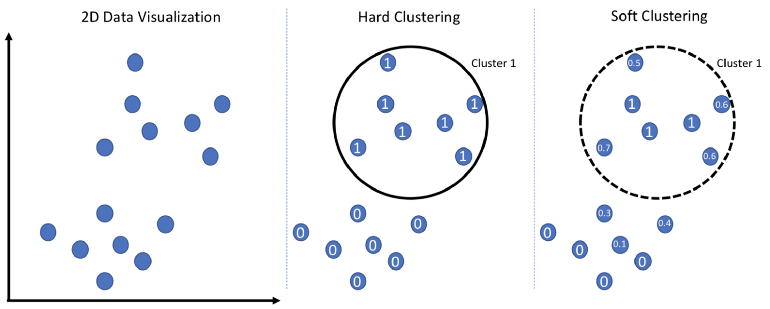
\includegraphics[width=\textwidth]{img/cmeans_explanation.png}
                \caption
                {Zobrazowanie róźnicy między działaniem KMeans a CMeans \cite{cmeans_desc_img}}
                \label{fig:cmeans_expl}
            \end{figure}
            \FloatBarrier
        }
    }

    \section{Eksperymenty} {

        \subsection{Zbiór mammography} {

            \begin{figure}[!htbp]
                \centering
                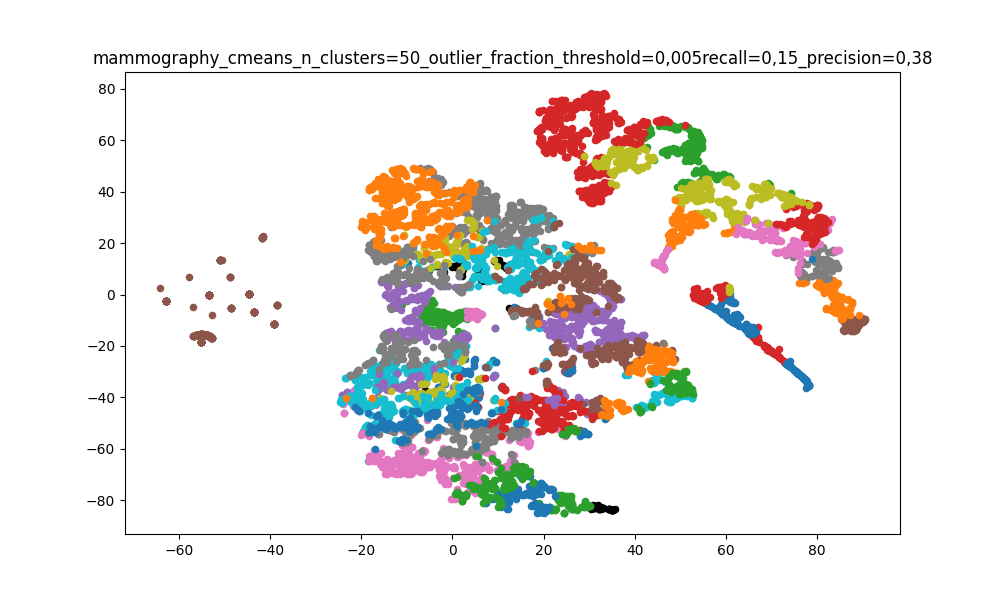
\includegraphics[width=\textwidth]{img/mammography_cmeans_n_clusters=50_outlier_fraction_threshold=0,005-182204.png}
                \caption{}
                \label{fig:mamm_cmeans}
            \end{figure}

            \begin{figure}[!htbp]
                \centering
                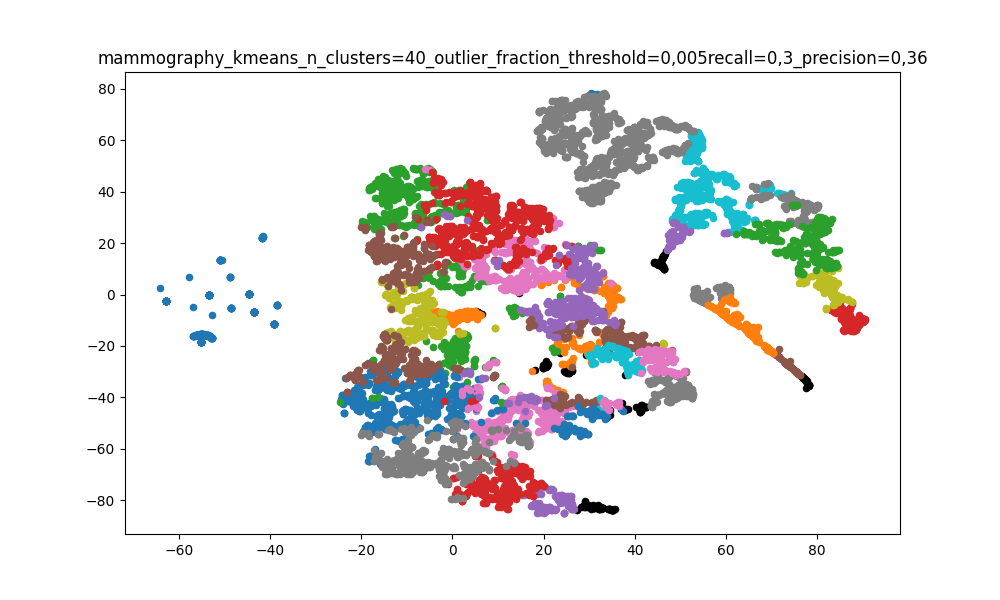
\includegraphics[width=\textwidth]{img/mammography_kmeans_n_clusters=40_outlier_fraction_threshold=0,005-182326.png}
                \caption{}
                \label{fig:mamm_kmeans}
            \end{figure}

            \begin{table}[!htbp]
                \footnotesize
                \centering
                \begin{tabular}{|c|c|c|c|c|c|}
                    \hline
                    algorytm & zbiór & liczba klastrór & próg wykrywania & recall & precision \\ \hline
                    cmeans & mammography & 40 & 0.005 & 0.15 & 0.25 \\
                    cmeans & mammography & 50 & 0.005 & 0.15 & 0.38 \\ \hline
                    kmeans & mammography & 40 & 0.005 & 0.3 & 0.36 \\
                    kmeans & mammography & 50 & 0.005 & 0.27 & 0.29 \\ \hline
                \end{tabular}
                \caption
                {Zestawienie wyników działania algorytmów dla zbioru mammography}
                \label{tab:mamm}
            \end{table}
            \FloatBarrier
        }

        \subsection{Zbiór synthetic} {

            \begin{table}[!htbp]
                \footnotesize
                \centering
                \begin{tabular}{|c|c|c|c|c|c|}
                    \hline
                    Algorytm & Zbiór & liczba klastrór & próg wykrywania & recall & precision \\ \hline
                    cmeans & synthetic & 2 & 0.1 & 0.85 & 1.0 \\
                    cmeans & synthetic & 2 & 0.2 & 0.85 & 1.0 \\
                    cmeans & synthetic & 5 & 0.1 & 0.9 & 1.0 \\
                    cmeans & synthetic & 5 & 0.2 & 0.9 & 1.0 \\
                    cmeans & synthetic & 10 & 0.01 & 0.0 & 0.0 \\
                    cmeans & synthetic & 10 & 0.1 & 0.9 & 1.0 \\
                    cmeans & synthetic & 10 & 0.2 & 1.0 & 0.13 \\
                    cmeans & synthetic & 15 & 0.01 & 0.0 & 0.0 \\
                    cmeans & synthetic & 15 & 0.1 & 0.95 & 0.2 \\
                    cmeans & synthetic & 15 & 0.2 & 1.0 & 0.1 \\
                    cmeans & synthetic & 20 & 0.01 & 0.15 & 1.0 \\
                    cmeans & synthetic & 20 & 0.1 & 1.0 & 0.15 \\
                    cmeans & synthetic & 20 & 0.2 & 1.0 & 0.1 \\ \hline
                    kmeans & synthetic & 2 & 0.1 & 0.9 & 1.0 \\
                    kmeans & synthetic & 2 & 0.2 & 0.9 & 1.0 \\
                    kmeans & synthetic & 5 & 0.1 & 0.9 & 1.0 \\
                    kmeans & synthetic & 5 & 0.2 & 0.9 & 1.0 \\
                    kmeans & synthetic & 10 & 0.01 & 0.05 & 1.0 \\
                    kmeans & synthetic & 10 & 0.1 & 0.95 & 1.0 \\
                    kmeans & synthetic & 10 & 0.2 & 0.95 & 1.0 \\
                    kmeans & synthetic & 15 & 0.01 & 0.15 & 1.0 \\
                    kmeans & synthetic & 15 & 0.1 & 0.95 & 0.56 \\
                    kmeans & synthetic & 15 & 0.2 & 0.95 & 0.2 \\
                    kmeans & synthetic & 20 & 0.01 & 0.3 & 1.0 \\
                    kmeans & synthetic & 20 & 0.1 & 0.95 & 0.3 \\
                    kmeans & synthetic & 20 & 0.2 & 1.0 & 0.1 \\ \hline
                \end{tabular}
                \caption
                {Zestawienie wyników działania algorytmów dla zbioru synthetic}
                \label{tab:synth}
            \end{table}

            \begin{figure}[!htbp]
                \centering
                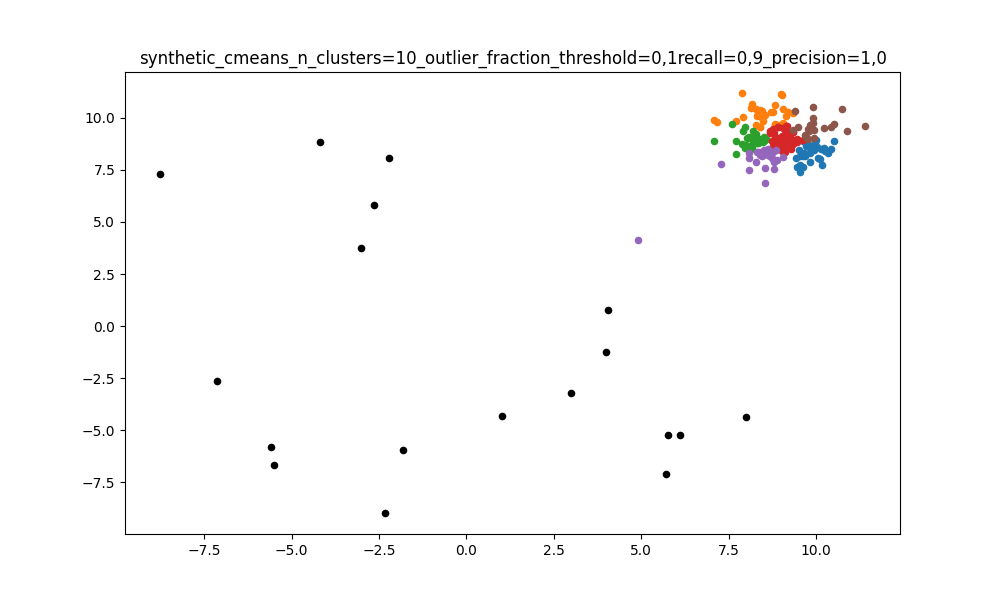
\includegraphics[width=\textwidth]{img/synthetic_cmeans_n_clusters=10_outlier_fraction_threshold=0,1-182007.png}
                \caption{}
                \label{fig:synth_cmeans}
            \end{figure}

            \begin{figure}[!htbp]
                \centering
                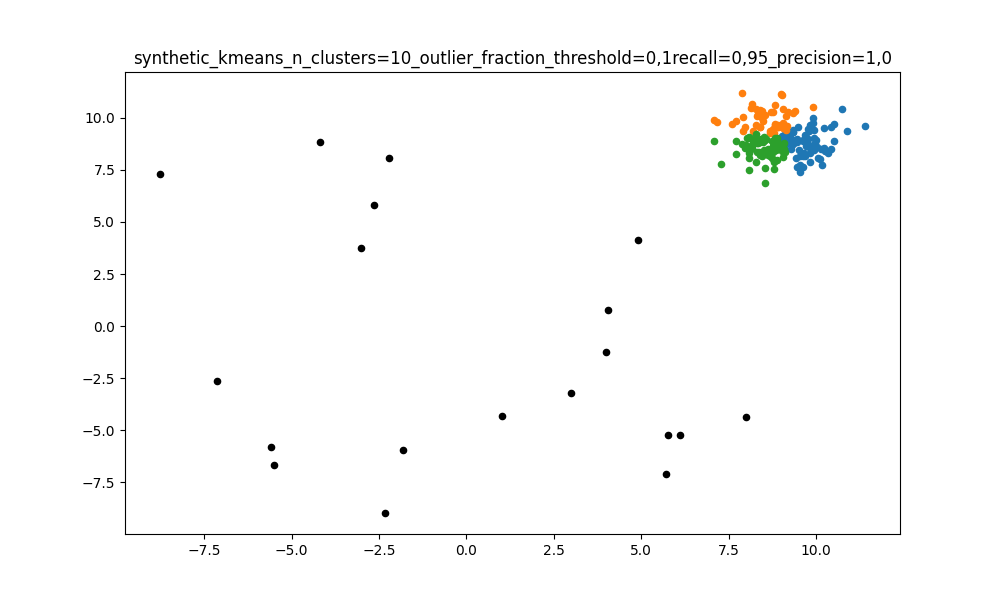
\includegraphics[width=\textwidth]{img/synthetic_kmeans_n_clusters=10_outlier_fraction_threshold=0,1-182011.png}
                \caption{}
                \label{fig:synth_kmeans}
            \end{figure}
            \FloatBarrier
        }

        \subsection{Zbiór http} {

            \begin{figure}[!htbp]
                \centering
                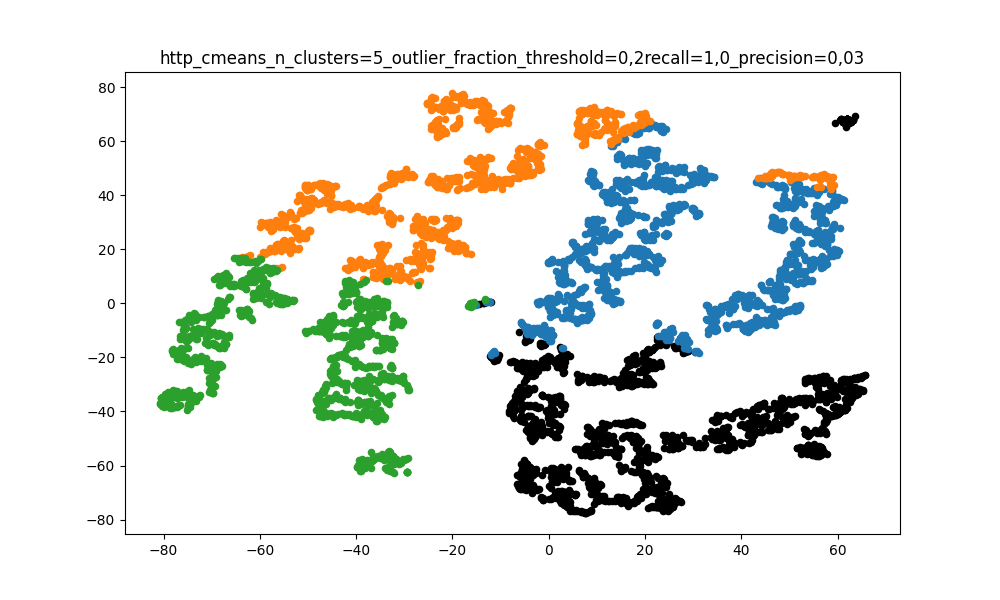
\includegraphics[width=\textwidth]{img/http_cmeans_n_clusters=5_outlier_fraction_threshold=0,2-183301.png}
                \caption{}
                \label{fig:http_cmeans}
            \end{figure}

            \begin{figure}[!htbp]
                \centering
                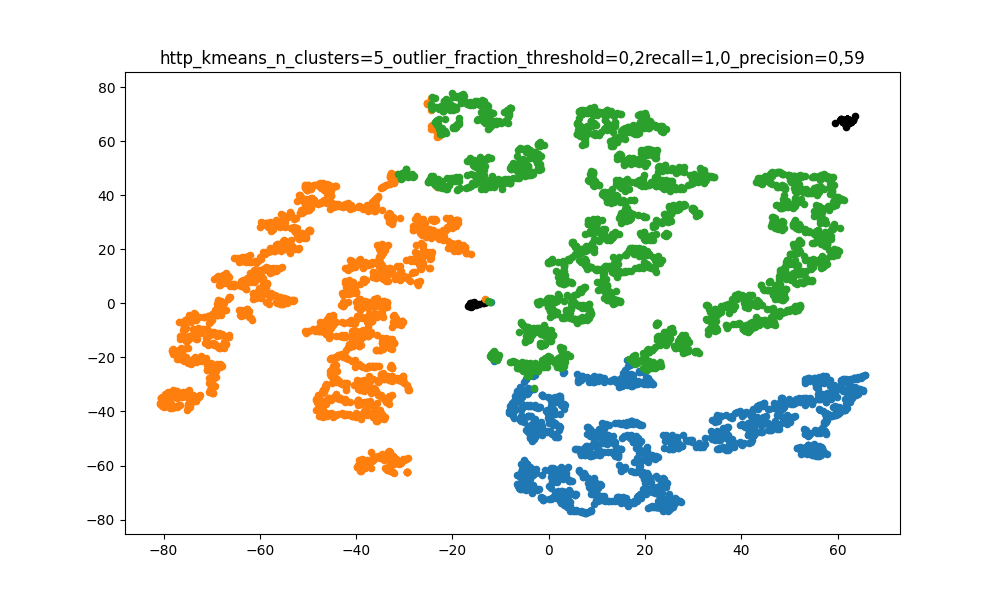
\includegraphics[width=\textwidth]{img/http_kmeans_n_clusters=5_outlier_fraction_threshold=0,2-183849.png}
                \caption{}
                \label{fig:http_kmeans}
            \end{figure}

            \begin{table}[!htbp]
                \footnotesize
                \centering
                \begin{tabular}{|c|c|c|c|c|c|}
                    \hline
                    algorytm & zbiór & liczba klastrór & próg wykrywania & recall & precision \\ \hline
                    cmeans & http & 5 & 0.1 & 0.0 & 0.0 \\
                    cmeans & http & 5 & 0.2 & 1.0 & 0.03 \\
                    cmeans & http & 8 & 0.01 & 0.0 & 0.0 \\
                    cmeans & http & 8 & 0.05 & 0.0 & 0.0 \\
                    cmeans & http & 10 & 0.01 & 0.0 & 0.0 \\
                    cmeans & http & 10 & 0.05 & 0.0 & 0.0 \\
                    cmeans & http & 10 & 0.1 & 1.0 & 0.03 \\
                    cmeans & http & 10 & 0.2 & 1.0 & 0.01 \\
                    cmeans & http & 15 & 0.05 & 0.0 & 0.0 \\
                    cmeans & http & 15 & 0.1 & 1.0 & 0.01 \\
                    cmeans & http & 20 & 0.01 & 0.0 & 0.0 \\
                    cmeans & http & 20 & 0.05 & 1.0 & 0.02 \\ \hline
                    kmeans & http & 5 & 0.1 & 1.0 & 0.59 \\
                    kmeans & http & 5 & 0.2 & 1.0 & 0.59 \\
                    kmeans & http & 8 & 0.01 & 1.0 & 0.55 \\
                    kmeans & http & 8 & 0.05 & 1.0 & 0.55 \\
                    kmeans & http & 10 & 0.01 & 1.0 & 0.55 \\
                    kmeans & http & 10 & 0.05 & 1.0 & 0.13 \\
                    kmeans & http & 10 & 0.1 & 1.0 & 0.13 \\
                    kmeans & http & 10 & 0.2 & 1.0 & 0.01 \\
                    kmeans & http & 15 & 0.05 & 1.0 & 0.16 \\
                    kmeans & http & 15 & 0.1 & 1.0 & 0.03 \\
                    kmeans & http & 20 & 0.01 & 1.0 & 0.51 \\
                    kmeans & http & 20 & 0.05 & 1.0 & 0.12 \\ \hline
                \end{tabular}
                \caption
                {Zestawienie wyników działania algorytmów dla zbioru http}
                \label{tab:http}
            \end{table}
            \FloatBarrier
        }
    }

    \section{Dyskusja i wnioski} {
        Analizując uzyskane wyniki można stwierdzić, że wyniki uzyskane dla zbioru
        \textit{synthetic} są dosyć zbliżone z tendencją, że dla algorytmu KMeans
        uzyskano nieznacznie lepsze wyniki. Na rysunkach \ref{fig:synth_cmeans} oraz
        \ref{fig:synth_kmeans} zostały przedstawione dwie wybrane wizualicje, które
        cechowały się najwyższymi wartościami recall i precision. Analizując te rysunki
        można zauwazyć, że dla KMeans widoczna jest mniejsza liczba kolorów co świadczy
        o tym innym sposobie klasteryzacji - soft clustering w zwartej liczbie punktów
        oznaczył więcej klastrów. Można też zauważyć jeden punkt na rysynku
        \ref{fig:synth_cmeans}, który powinien byc oznaczony w klastrze z wyjątkami
        lecz został oznaczony w innym klastrze, najprawdopodobniej przez wartość poziomu
        przynaleźności. Poskutowało to bezpośrednio róźnicą w wartości recall na
        poziomie 0.05.

        Co więcej warto zaznaczyć, że w przypadku pozostałych zbiorów, które posiadają
        więcej niż dwa wymiary, do wizualizacji został wykorzystany \textit{TSNE}
        (ang. T-distributed Stochastic Neighbor Embedding) \cite{tsne}. Przechodząc do
        zbioru \textit{mammography}, warto zaznaczyć, że zostały wykonane eksperymenty dla
        zróżniociowanych parametrów jednak tylko dla przedstawionych w tabeli
        \ref{tab:mamm} udało się uzyskać w miarę zadawalające wyniki. W przypadku
        innych testowanych wartości dla tego zbioru, wyniki zarówno dla KMeans oraz
        CMeans były identycznie i niezadawalające tzn. \textit{recall=0.0} oraz
        \textit{precision=0.0}, wiec nie można było na ich podstawie wykazać dominacji
        jednego algorytmu na drugim przy takim samym zbiorze danych oraz parametrach.
        Skupiając sie jednak na wynikach przedstawionych w \ref{tab:mamm} oraz
        wizualizacjach najlepszych wyników ukazanych na rysunkach \ref{fig:mamm_cmeans}
        oraz \ref{fig:mamm_kmeans} można stwierdzić, że ponownie algorytm KMeans okazał
        się być skuteczniejszy. Wartość recall dla CMeans jest dwukrotnie mniejsza
        natomiast z pozytywów można zauważyć to, że precision jest o 0.02 wyższe. W
        omawianych przypadkach najlepszych wyników, które zostały przedstawione na
        rysunkach warto zwrócić uwagę na różne wartości liczby klastrów. Jest to
        odpowiednio dla CMeans 50 natomiast dla KMeans 40.

        Skupiając się na ostatnim zbiorze a mianowicie \textit{http} niestety musimy
        się przyznać do porażki, gdyż dla żadnych wartości parametrów nie udało uzyskać
        się zadowalających wyników dla badanego algorytmu czyli CMeans. Ze względu na
        wielokrotne wykorzystanie tego zbioru oraz wcześniejsze wykorzystanie KMeans
        były znane w miarę optymalne wartości. Niestety dla CMeans totalnie się one nie
        sprawdzały. Eksperymenty były przeprowadzone masowo poprzez wielkrotne
        uruchomienia dla różnych parametrów, dostosowywyjąc je na podstawie obserwacji
        z poprzednich podgrup eksperymentów. Była też wyznaczana dla wszystkich zbiorów
        optymalna liczba klastrów metodą łokcia (ang. Elbow Method) natomiast to też w
        przypadku zbioru \textit{http} oraz algorytmu CMeans nie przyniosło
        oczekiwanych efektów. Co warto dodać, algorytm KMeans dla dużo wyższej liczby
        klastrów tj. około 40 również drastycznie pogarszał wyniki. Co więcej same
        parametry były dopiero pamiętając o tym, że bezpośrednio od siebie zależą tzn.
        parametr \textit{próg wykrywania} działa w sposób następujący, że jeżeli liczność
        elementów w klastrze jest poniżej jego wartości są uznawane za wyjątki.
        Oczywiście wartość tego parametru jest to wartość z zakresu
        \textit{(0,1) * wielkość zbioru danych}.

        Podsumowując, algorytm \textit{CMeans} jest ciekawym i nowatorskim rozwiązaniem
        natomiast w przypadku użytych zbiorów danych, w szczególności tych naturalnych
        nie wykazał swej ponadmiarowej skuteczności w porównaniu z algorytmem
        \textit{KMeans}.
    }

    \begin{thebibliography}{0}
        \bibitem{fuzzy_c_means}{https://pypi.org/project/fuzzy-c-means/}
        \bibitem{sklearn}{https://scikit-learn.org/stable/}
        \bibitem{pyod}{https://pyod.readthedocs.io/en/latest/}
        \bibitem{odds}{http://odds.cs.stonybrook.edu/}
        \bibitem{cmeans_desc}{https://towardsdatascience.com/fuzzy-c-means-clustering-with-python-f4908c714081}
        \bibitem{cmeans_desc_img}{https://miro.medium.com/max/770/1*O5Ynz1UI6ClCs-Bdf-MG9A.png}
        \bibitem{tsne}{https://scikit-learn.org/stable/modules/generated/sklearn.manifold.TSNE.html}
    \end{thebibliography}

\end{document}
